%In this section, we present the MPC-based economic dispatch problem that we consider and provide the outline of the proposed methodology.

%\subsection{Economic dispatch problem}
%\paragraph*{Graph representation of the network}
%We formulation of the economic dispatch problem is provided, following the model of the network. 

Let a distribution power network be represented by the undirected and connected graph $\mathcal{G}=(\mathcal{N},\mathcal{E})$, where the set of busses is denoted by $\mathcal{N}=\{1,2,\dots,n\}$ and the set of edges that connect the busses is denoted by $\mathcal{E}$, i.e., $\mathcal{E}=\{(i,j):i,j\in\mathcal{N} \}\subseteq\mathcal{N}\times\mathcal{N}$. Furthermore, the set of neighbor busses of bus $i$ is denoted by $\mathcal{N}_i$, i.e., $\mathcal{N}_i = \{j:(i,j)\in \mathcal{E} \}$. Each bus $i$ might contain an aggregate load (power demand), dispatchable or nondispatchable distributed generation units, and energy storage devices. Each of these components has operational constraints, which are assumed to be polyhedral and compact. Furthermore, each bus $i \in \mathcal{N}$ also considers power balance equations that must be satisfied  at each iteration $k$, as follows: 
\begin{align}
u^{\mathrm{g}}_{i,k} + u^{\mathrm{st}}_{i,k} + u^{\mathrm{m}}_{i,k} + \sum_{j \in \mathcal{N}_i} v^{j}_{i,k} - {d}_{i,k}=0,  \label{eq:lo_pb}\\
v^{j}_{i,k} + v^{i}_{j,k} = 0, \quad \forall j \in \mathcal{N}_i, \label{eq:coup_pb}
\end{align}
where  ${u}_{i,k}^{\mathrm{g}}\in \mathbb{R}$, $u^{\mathrm{st}}_{i,k}\in \mathbb{R}$, and $u_{i,k}^{\mathrm{m}} \in \mathbb{R}_{\geq 0}$ denote the power generated from dispatchable unit, delivered from/to storage unit, and imported from the main grid if connected, respectively.  %Note that bus $i$ belongs to the set of busses that are connected to the main grid, denoted by $\mathcal{N}^{\mathrm{m}}$, and 
Furthermore, $d_{i,k}\in \mathbb{R}$ denotes the difference between uncertain loads and the power generated from non-dispatchable units, which is also uncertain. Additionally, $v_{i,k}^{j} \in \mathbb{R}$ denotes the power transferred to/from the neighbor bus $j  \in \mathcal{N}_i$. Equation \eqref{eq:lo_pb} can be considered as a local power balance, whereas \eqref{eq:coup_pb} couples two neighboring busses.

The variable $d_{i,k}$ is considered to be uncertain and its disturbance is bounded, i.e.,
\begin{align}
{d}_{i,k}&=\hat{d}_{i,k} + w_{i,k}^{\mathrm{d}}, \quad \forall i \in \mathcal{N}, \label{eq:ul}\\
|w_{i,k}^{\mathrm{d}}| &\leq \bar{w}_{i}^{\mathrm{d}}, \quad \forall i \in \mathcal{N}, \label{eq:w_ul}
\end{align}
where  $\hat{d}_{i,k}$ denotes the forecast of $d_{i,k}$ whereas  $w_{i,k}^{\mathrm{d}} \in \mathbb{R}$ and $\bar{w}_{i}^{\mathrm{d}} \in \mathbb{R}$  represent the disturbance/uncertainty and its bound, which is assumed to be known, for simplicity and since this work does not focus on handling uncertainties. A stochastic method such as the ones presented in \cite{margellos2014,ananduta2019b} can be considered as an extension. % We assume that the forecast, $\hat{d}_{i}$, can be obtained and  the disturbance, $w_{i,k}^{\mathrm{d}}$, is bounded, i.e.,
%\begin{equation}

%\end{equation}
%where $\bar{w}_{i}^{\mathrm{d}} \in \mathbb{R}_{\geq 0}$ denotes the bound of $w_{i,k}^{\mathrm{d}}$ and is assumed to be known. 
%\paragraph*{Distributed generation units.} 


  % For an economic dispatch problem, these components are modeled next.

To state the MPC-based economic dispatch problem, define the vectors of decision variables of each bus $i\in \mathcal{N}$, which correspond to active components, by $\bm{u}_{i,k} = \begin{bmatrix}
u^{\mathrm{st}}_{i,k} & u^{\mathrm{g}}_{i,k}  & u^{\mathrm{m}}_{i,k}
\end{bmatrix}^{\top} \in \mathbb{R}^{3}$ and $\bm{v}_{i,k} = \begin{bmatrix}
v_{i,k}^{j}
\end{bmatrix}_{i\in \mathcal{N}_i}^{\top} \in \mathbb{R}^{|\mathcal{N}_i|}$. 
\iffalse  
%\paragraph*{Loads.}
The demand of each bus $i\in\mathcal{N}$ is considered to be uncertain, i.e.,
\begin{equation}
{d}_{i,k}=\hat{d}_{i,k} + w_{i,k}^{\mathrm{d}}, \quad \forall i \in \mathcal{N}, \label{eq:ul}
\end{equation}
where  ${d}_{i,k}, \hat{d}_{i} \in \mathbb{R}_{\geq 0}$ denote the uncertain demand of bus $i$ and its forecast, respectively, while  $w_{i,k}^{\mathrm{d}} \in \mathbb{R}$ represent the disturbance/uncertainty of the load. Furthermore, we assume that the demand forecast, $\hat{d}_{i}$, can be obtained and  the disturbance, $w_{i,k}^{\mathrm{d}}$, is bounded, i.e.,
\begin{equation}
|w_{i,k}^{\mathrm{d}}| \leq \bar{w}_{i}^{\mathrm{d}}, \quad \forall i \in \mathcal{N}, \label{eq:w_ul}
\end{equation}
where $\bar{w}_{i}^{\mathrm{d}} \in \mathbb{R}_{\geq 0}$ denotes the bound of $w_{i,k}^{\mathrm{d}}$ and is assumed to be known. 
%\paragraph*{Distributed generation units.} 
The power produced by non-dispatchable distributed generation units, e.g.,  solar-based and wind-based power, is modeled similarly as uncertain loads. Denote the power produced by such generation units by ${u}_{i,k}^{\mathrm{nd}}\in \mathbb{R}_{\geq 0}$, its forecast by $\hat{u}_{i,k}^{\mathrm{nd}} \in \mathbb{R}_{\geq 0}$, its uncertainty by $w_{i,k}^{\mathrm{nd}} \in \mathbb{R}$, and the bound of its uncertainty by $\bar{w}_{i}^{\mathrm{nd}}$. The non-dispatchable power production is represented as follows:
\begin{align}
{u}_{i,k}^{\mathrm{nd}}&=\hat{u}_{i,k}^{\mathrm{nd}} + w_{i,k}^{\mathrm{nd}},  &\forall i \in \mathcal{N}, \label{eq:re}\\
|w_{i,k}^{\mathrm{nd}}| &\leq \bar{w}_{i}^{\mathrm{nd}} ,  &\forall i \in \mathcal{N}. \label{eq:w_re}
\end{align}
Note that if at bus $i$ there does not exists a non-dispatchable generation unit, then $\hat{u}_{i,k}^{\mathrm{nd}}=0$, for any $k\geq0$, and $\bar{w}_{i}^{\mathrm{nd}}=0$. We also assume that the forecast and the bound, $\bar{w}_{i}^{\mathrm{nd}}$, can be obtained. On the other hand, the dispatchable generators are modeled by production capacity constraints as follows:
\begin{equation}
0 \leq {u}_{i,k}^{\mathrm{g}} \leq \bar{u}_{i}^{\mathrm{g}},  \quad \forall i \in \mathcal{N}^{\mathrm{dg}}, \label{eq:p_g}
\end{equation}
where ${u}_{i,k}^{\mathrm{g}}$ denotes the power produced by the dispatchable generator at bus $i$, $\bar{u}_{i,k}^{\mathrm{g}}$ denotes the maximum production capacity, and $\mathcal{N}^{\mathrm{dg}} \subset \mathcal{N}$ denotes the set of busses that have dispatchable generation units. 
%\paragraph*{Energy storage devices.}  
Furthermore, denote the set of busses where the storage devices are installed by $\mathcal{N}^{\mathrm{st}} \subset \mathcal{N}$. The dynamics of a storage device at bus $i \in \mathcal{N}^{\mathrm{st}}$ is represented as a simple integrator model with the following discrete-time state-space equation:
\begin{equation}
x_{i,k+1} = a_i x_{i,k} + b_i u^{\mathrm{st}}_{i,k}, \label{eq:dyn_bat}
\end{equation}
where $x_{i,k} \in \mathbb{R}_{\geq 0}$ denotes the state-of-charge (SoC) of the storage device, $u^{\mathrm{st}}_{i,k} \in \mathbb{R}$ denotes the power delivered to/from the storage, $a_i \in (0,1]$ denotes the efficiency of the storage and $b_i~=~-\frac{T_{\mathrm{s}}}{e_{\mathrm{cap},i}}$, where $T_{\mathrm{s}}$ and $e_{\mathrm{cap},i}$ denote the sampling time and the maximum capacity of the storage, respectively. Note that $u^{\mathrm{st}}_{i,k}$ represents both the charging and discharging power since we want to avoid the hybrid dynamics that are implied if we distinguish them and introduce the charging/discharging efficiencies as in \cite{garcia2015,garcia2016}. Furthermore, the operational limits of the storage units are represented by the following constraints:
\begin{align}
x^{\mathrm{min}}_i &\leq x_{i,k} \leq x^{\mathrm{max}}_i,  \label{eq:cap_bat}\\
-u^{\mathrm{ch}}_i &\leq u^{\mathrm{st}}_{i,k} \leq u^{\mathrm{dh}}_i,\label{eq:ch_bat}
\end{align}
where $x^{\mathrm{min}}_i,x^{\mathrm{max}}_i  \in [0,1]$  denote the minimum and the maximum SoC of the storage of microgrid $i$, respectively.  Moreover, $u^{\mathrm{ch}}_i \in \mathbb{R}_{\geq 0}$ and $u^{\mathrm{dh}}_i \in \mathbb{R}_{\geq 0}$ denote the maximum charging and discharging power of the storage. 
%\paragraph{Electrical vehicles} It is considered that an electrical vehicle can work as a power source or as a load. Therefore, denote the agregated power that is delivered to/from electric vehicles at bus $i \in \mathcal{N}$ by $p_{i,k}^{\mathrm{ev}} \in \mathbb{R}$. It is assumed that the mode and the amount of power delivered to/from are made by the local controller of each vehicle and can be communicated. 
%\begin{remark}
%	The amount of controllable loads and power delivered to/from electrical vehicles might also be included as decision variables in the economic dispatch problem. However, this inclusion requires a more complex model of the loads and electrical vehicles. In this regard, the proposed approach can also be extended to such cases. \eod
%\end{remark}
%\paragraph*{power balance equations at each bus}
 %Additionally, $p_{i,k}^{\mathrm{im}}$ and $p_{ij,k}^{\mathrm{t}}$ are constrained, as follows:
%\begin{align}
%	0 &\leq p_{i,k}^{\mathrm{im}} \leq \bar{p}_{i,k}^{\mathrm{im}}, \label{eq:p_im} \\
%-\bar{p}_{ij,k}^{\mathrm{t}} &\leq p_{ij,k}^{\mathrm{t}} \leq \bar{p}_{ij,k}^{\mathrm{t}}, \quad \forall j \in \mathcal{N}_i, \label{eq:p_t}
%\end{align}
%where $\bar{p}_{i,k}^{\mathrm{im}},\bar{p}_{ij,k}^{\mathrm{t}} \in \mathbb{R}_{\geq 0}$ denote the maximum power can be imported from the main grid and the maximum power can be transferred to/from bus $j$, respectively.

%\paragraph*{economic dispatch problem formulation}
Now, we are in a position to state the economic dispatch problem of the network based on an MPC formulation. Firstly, we robustify the decisions by considering the worst-case scenario of the disturbances as follows: 
\begin{equation}
w_{i,k}^{\mathrm{l}} = \bar{w}_{i}^{\mathrm{l}}, \quad 
w_{i,k}^{\mathrm{nd}} = -\bar{w}_{i}^{\mathrm{nd}}, \quad \forall i \in \mathcal{N}. \label{eq:ws_d}
\end{equation}
Secondly, define the vector of decision variables of each bus $i\in \mathcal{N}$ by $\bm{u}_{i,k} = \begin{bmatrix}
u^{\mathrm{st}}_{i,k} & u^{\mathrm{g}}_{i,k}  & u^{\mathrm{m}}_{i,k}
\end{bmatrix}^{\top} \in \mathbb{R}^{3}$ and $\bm{v}_{i,k} = \begin{bmatrix}
v_{i,k}^{j}
\end{bmatrix}_{i\in \mathcal{N}_i}^{\top} \in \mathbb{R}^{|\mathcal{N}_i|}$. In this regard, the following additional constraints must be imposed:
\begin{equation}
\begin{aligned}
&u_{i,k}^{\mathrm{g}}=0, \ \forall i \notin \mathcal{N}^{\mathrm{dg}}, \quad u_{i,k}^{\mathrm{st}}=0, \ \forall i \notin \mathcal{N}^{\mathrm{st}}, \\ &u_{i,k}^{\mathrm{m}}=0, \ \forall i \notin \mathcal{N}^{\mathrm{m}}. 
\end{aligned}
\label{eq:0_const}
\end{equation}
Thirdly, 
\fi 
Furthermore, an economic quadratic cost function is considered as follows:
\begin{equation}
J_{i,k}(\bm{u}_{i,k},\bm{v}_{i,k}) = \bm{u}_{i,k}^{\top}R_i\bm{u}_{i,k}+ \bm{v}_{i,k}^{\top}Q_i\bm{v}_{i,k}, \label{eq:cost_func}
\end{equation}
where $R_i$ and $Q_i$ are positive definite diagonal matrices of suitable dimensions. Therefore, the optimization problem behind an MPC-based economic dispatch is stated as follows:
\begin{subequations}
	\begin{align}
&	\min_{\{\{(\bm{u}_{i,\ell},\bm{v}_{i,\ell})\}_{i \in \mathcal{N}}\}_{\ell=k}^{k+h-1}} \sum_{i \in \mathcal{N}} \sum_{\ell =k}^{k+h-1}  J_{i,\ell}(\bm{u}_{i,\ell},\bm{v}_{i,\ell}) \label{eq:net_cost_func}\\
& \qquad \qquad	\text{s.t. }   
	 (\bm{u}_{i,\ell},\bm{v}_{i,\ell}) \in \mathcal{P}_i, \ \forall i \in \mathcal{N}, \label{eq:net_loc_cons}\\
	&  \qquad \qquad \qquad  v_{i,\ell}^j + v_{j,\ell}^i = 0, \ \forall j\in\mathcal{N}_i, \ \ \forall i \in \mathcal{N}, \label{eq:net_coup_cons}
	\end{align}
	\label{eq:MPC_net}%
\end{subequations}
for all $\ell \in \{k,\dots,k+h-1\}$, where $h \in \mathbb{Z}_{\geq 1}$ denotes the prediction horizon. The set $\mathcal{P}_i\subset \mathbb{R}^{3+|\mathcal{N}_i|}$, for each $i\in\mathcal{N}$, is assumed to be a compact polyhedral set such that \eqref{eq:lo_pb}, \eqref{eq:ul}, and \eqref{eq:w_ul} as well as the operational constraints of the active components hold. We refer to \cite{ananduta2019a} for a more detailed description of such operational constraints. %,\eqref{eq:p_im}-\eqref{eq:rw_re}
%On the other hand, the coupled constraints \eqref{eq:net_coup_cons} with the appropriate matrices $\bm{G}_{ij}$, for all $j\in\mathcal{N}_i$, are constructed from \eqref{eq:coup_pb}. 

\color{black}
\begin{assum}\label{as:feas_ED_cent}
	For each $k \in \mathbb{Z}_{\geq 0}$, a feasible set of Problem \eqref{eq:MPC_net} exists. %\eod
\end{assum}


\begin{rem} 	Assumption 1 is considered in order to ensure that the proposed scheme obtains a solution. In practice, the satisfaction of this assumption is achieved either if the network is connected with the main grid, which is usually assumed as an infinite source of power, or if it is not connected with the main grid, the total power that can be generated by the distributed generators is sufficiently larger than the loads within the network.
\end{rem}

%\begin{rem}
%	Since the main focus of this paper is not on how to handle uncertainties, we consider that the bounds of the uncertain variables are known for simplicity. However, a stochastic method such as the ones presented in \cite{margellos2014,velarde2017} can also be implemented to relax this assumption. A stochastic formulation using the method presented in \cite{margellos2014} for a similar economic dispatch problem can be found in \cite{ananduta2019b}. \eod
%\end{rem}


%\subsection{Outline of the proposed method}

%\color{blue}
In this paper, we solve Problem \eqref{eq:MPC_net} in a non-centralized fashion, where there exists $m$ local controllers. Thus, the network must be partitioned into $m$ sub-systems, each of which is assigned to a local controller. \color{black}Then, the controllers cooperatively solve Problem \eqref{eq:MPC_net}. To that end, Problem \eqref{eq:MPC_net}, which has coupling constraints \eqref{eq:net_coup_cons}, must be decomposed. Our main idea is to decompose Problem \eqref{eq:MPC_net} into a number of sub-problems, not larger than $m$, such that each sub-problem can be solved independently. As we will show in the next sections, the independence of each sub-problem depends on the self-sufficiency of the microgrids, i.e., the ability to meet local load using local production. Therefore, we propose an event-triggered repartitioning and coalition formation procedures to obtain self-sufficient partitions. %Therefore, firstly, we propose a repartitioning procedure with the aim of obtaining self-sufficient and efficient microgrids. Since the load and the power production of a non-dispatchable generation unit are uncontrollable and vary over time, the network might need to be repartitioned to maintain self-sufficiency. %In this regard, the repartitioning of the network is event-triggered. 
%Secondly, we propose a coalition-based economic dispatch approach to solve Problem \eqref{eq:MPC_net}. The approach is based on forming self-sufficient coalitions of microgrids, thus requiring a coalition formation algorithm. In this method, each coalition independently solves its own local economic dispatch problem, which is a sub-problem of \eqref{eq:MPC_net}. 
A flow diagram that summarizes the overall method is shown in Figure \ref{fig:prop_sch}. 
% \iffalse 
\begin{figure}
	\centering
	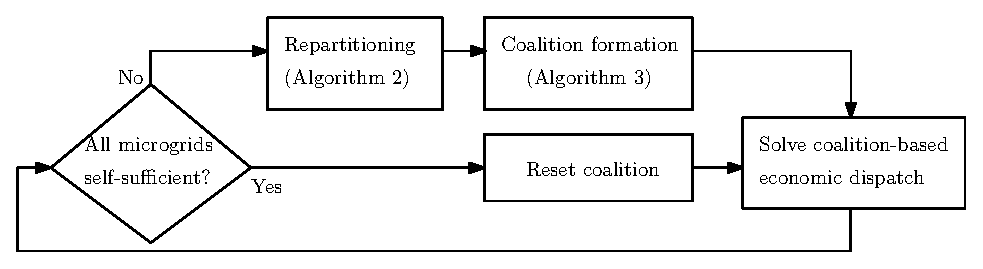
\includegraphics[scale=0.5]{img/ov_sch}
	\caption{The overall scheme of the proposed method.
	}
	\label{fig:prop_sch}
\end{figure}
%\fi
%\paragraph*{the goals} 


 
%\paragraph*{Reformulate the economic dispatch problem}
%In this regard, as shown in Proposition \ref{lem:net2mg},  Problem \eqref{eq:MPC_net} is reformulated as an economic dispatch problem of interconnected microgrids. 